%; whizzy chapter -dvi
% -initex iniptex -latex platex -format platex -bibtex jbibtex -fmt fmt
% 以上 whizzytex を使用する場合の設定。
 
%     Tokyo Debian Meeting resources
%     Copyright (C) 2012 Junichi Uekawa
%     Copyright (C) 2011 Nobuhiro Iwamatsu

%     This program is free software; you can redistribute it and/or modify
%     it under the terms of the GNU General Public License as published by
%     the Free Software Foundation; either version 2 of the License, or
%     (at your option) any later version.

%     This program is distributed in the hope that it will be useful,
%     but WITHOUT ANY WARRANTY; without even the implied warranty of
%     MERCHANTABILITY or FITNESS FOR A PARTICULAR PURPOSE.  See the
%     GNU General Public License for more details.

%     You should have received a copy of the GNU General Public License
%     along with this program; if not, write to the Free Software
%     Foundation, Inc., 51 Franklin St, Fifth Floor, Boston, MA  02110-1301 USA

%  preview (shell-command (concat "evince " (replace-regexp-in-string "tex$" "pdf"(buffer-file-name)) "&"))

%%ここからヘッダ開始。

\documentclass[mingoth,a4paper]{jsarticle}
\usepackage{monthlyreport}
% 日付を定義する、毎月変わります。
\newcommand{\debmtgyear}{2014}
\newcommand{\debmtgmonth}{03}
\newcommand{\debmtgdate}{15}
% started from zero:
% (let ((year 2013) (month 7)) (+ (* (- year 2005) 12) month -1))
\newcommand{\debmtgnumber}{111}

\begin{document}

\begin{titlepage}
\thispagestyle{empty}
% タイトルページ:編集必要な部分は最初のマクロに飛ばすこと

\vspace*{-2cm}
第\debmtgnumber{}回 東京エリア Debian 勉強会資料\\
\hspace*{-2cm}

\includegraphics{image2012-natsu/dotdeb.pdf}\\
\hfill{}\debmtgyear{}年\debmtgmonth{}月\debmtgdate{}日

% ここはアップデートすること
% 全角文字にしないとフォントのサイズが合わないので注意
\rotatebox{10}{\fontsize{32}{32} {\gt 特集:iphone5を繋ぐ}}\\

\vspace*{-2cm}
\hfill{}
\includegraphics[height=6cm]{image200502/openlogo-nd.eps}
\end{titlepage}

\newpage

\begin{minipage}[b]{0.2\hsize}
 \definecolor{titleback}{gray}{0.9}
 \colorbox{titleback}{\rotatebox{90}{\fontsize{80}{80} {\gt デビアン勉強会} }}
\end{minipage}
\begin{minipage}[b]{0.8\hsize}
\hrule
\vspace{2mm}
\hrule
\begin{multicols}{2}
\tableofcontents
\end{multicols}
\vspace{2mm}
\hrule
\end{minipage}

\dancersection{事前課題}{野島 貴英}

今回の事前課題は以下です:
\begin{enumerate}
 \item 本日、何の作業をやるかを宣言ください。
\end{enumerate}
この課題に対して提出いただいた内容は以下です。
\begin{multicols}{2}
{\small
\begin{prework}{ 吉野(yy\_{}y\_{}ja\_{}jp) }
\begin{itemize}
\item manpages-ja 続き
\item DDTSS
\end{itemize}
\end{prework}

\begin{prework}{ dictoss(杉本 典充) }
 git-buildpackageでパッケージをつくれるように勉強する。
\end{prework}

\begin{prework}{ umireon }
 vagrantのbaseboxを作ります。
\end{prework}

\begin{prework}{ 野首 }
\begin{itemize}
\item KAKASI 2.3.6のリリースに向けた作業
\item LanguageToolのルール追加
\item navi2ch texiの確認
\item gnu.org web翻訳
\end{itemize}
\end{prework}

\begin{prework}{ 野島 }
 今度こそ、bitblockerでガードされたUEFI仕様のwindows 7機材に
Debianをデュアルブートインストール。
\end{prework}

}
\end{multicols}

\dancersection{Debian Trivia Quiz}{野島 貴英}

ところで、みなさん Debian 関連の話題においついていますか?Debian関連の話
題はメーリングリストをよんでいると追跡できます。ただよんでいるだけではは
りあいがないので、理解度のテストをします。特に一人だけでは意味がわからな
いところもあるかも知れません。みんなで一緒に読んでみましょう。

今回の出題範囲は\url{debian-devel-announce@lists.debian.org} や \url{debian-devel@lists.debian.org}に投稿された
内容などからです。

\begin{multicols}{2}
%; whizzy-master ../debianmeetingresume201311.tex
% 以上の設定をしているため、このファイルで M-x whizzytex すると、whizzytexが利用できます。
%

\santaku
{2014年GSoCのメンター募集が行われています。2014年のGSoCにて採択されていないものはどれ}
{hurd-i386の開発}
{clangでDebianのパッケージをコンパイルできるようにする}
{Android上でDebian環境を作れる件の改良を行う}
{A}
{他にもいろいろなProjectがDebian Projectから採択されています。Elektra\url{http://www.libelektra.org}で設定ファイルのアップグレードを改良するとか、libstdc++からlibc++を使うようにDebianを変更する件や、パッケージ管理にMuonを使う件など。参考:\url{https://wiki.debian.org/SummerOfCode2014/Projects}}

\santaku
{2014/2/14にバグレポートのIDが\#740000を向かえました。\#730000からどのぐらいの期間がたったでしょう?}
{1ヶ月と3日}
{3ヶ月と4日}
{10ヶ月と10日}
{B}
{毎年、Christian Perrierさんにより、バグレポートのIDについて、将来いつ何万番台を迎えるかについて当てるコンテストが行われています。}

\santaku
{Debianのコミュニティにより提供されているWebサービスについて調査が行われています。この調査の名前は?}
{Debian Services Servey}
{Outreach Program For Women}
{Debian Services Census}
{C}
{2014/2/13に呼びかけが行われました。現在のサービスの名前とURLのリストは、\url{https://wiki.debian.org/Services}にまとめられています。}

\santaku
{毎年恒例のDPL選挙が始まりました。2014年のDPL立候補者は誰?}
{Takahide Nojima}
{Lucas Nussbaum}
{Stefano Zacchiroli}
{B}
{lucusは2013年DPLですが、2年連続立候補となります。他の2名の方は、Gergely Nagyさん、Neil McGovernさんとなります。
 選挙期間は2014/3/31〜4/13となります。各候補者の声明は、\url{http://www.debian.org/vote/2014/platforms/}に掲載予定です。}

\end{multicols}

\dancersection{最近のDebian関連のミーティング報告}{野島 貴英}

\subsection{東京エリアDebian勉強会109回目報告}

 東京エリアDebian勉強会109回目は(株)スクウェア・エニックスさんで開催されました。
4名の参加者がありました。

\begin{itemize}
\item Debianにてdnsmasqを使い、複数のDebianの仮想環境を、モバイルPC上のDebian上で動かす際に便利な、
  \begin{itemize}
    \item 簡易DNSリゾルバの立て方、
    \item 簡易DNSサーバーの立て方、
    \item 5分でできる簡易PXE boot用サーバーの立て方
 \end{itemize}
について発表がありました。
\item 参加者全員で、各自の作業を行い、最後に成果発表をしました。
\end{itemize}

 宴会は会場近くの中華食べ放題「南国亭新宿店」にて行いました。

\subsection{東京エリアDebian勉強会110回目報告}

 第110回東京エリアDebian勉強会は、OSC 2014 Tokyo/Spring 出張編ということで
行われました。東京エリアDebian勉強会は2日目の3月1日(土)のみの出展でした。

\begin{itemize}
\item 場所は明星大学
\item iwamatsuさんにより、debian updateとdebianのEFI/UEFI対応について発表が行われました。
\item 展示について、iwamatsuさん、yy\_y\_ja\_jpさん、koedoyoshidaさん、野島で行いました。
\end{itemize}

% % (query-replace-regexp "<.*?>" "")
% % (query-replace-regexp "^[	 ]\+" "")

%-------------------------------------------------------------------------------
\dancersection{Debianでiphone5を繋ぐ}{野島 貴英}
%-------------------------------------------------------------------------------
\index{debian-iphon5}

\subsection{はじめに}

 大変不自由なスマートフォンなのに日本で驚異的に売れまくっているという、目を
被いたくなるような現実を作り出しているスマートフォンの1つとして、
iphone5があります\cite{iphone-japan-share}。このスマートフォン、
PCに繋ぐには、windows/macでiTuneなどの専用プロプリエタリなソフトウェアを
使ってデータ同期をしなければならないという、これでもかというぐらいの
不自由仕様となっています。

 ここでは、少しでもiphone5の不自由さを回避するため、

\begin{itemize}
\item 自由なDebianマシンに、なんとかして不自由なiphone5を繋ぐ事について、
\item iphone5がどのような仕組みでつながるのか(Debian開発者向け)
\end{itemize}

について述べます。

\subsection{本発表内容についての情報ソース}

 本発表内容の技術の情報ソースは、すべて

\begin{itemize}
\item Apple社のディベロッパーサイトで公開情報となっているもの(文献\cite{apple-fs-program-ref})
\item Debianパッケージに含まれるプログラムを解析した範囲
\item その他Webにて公開されている情報(文献\cite{usb-mux-desc},\cite{afc-desc},
\cite{iphone-hacking-accessories-desc})
\end{itemize}

のみに基づきます。

\subsection{Debianに繋ぐ}

 東京エリアDebian勉強会にいらっしゃるような方々は、普段から
Debian sidをお使いかと思いますので、ここでは、Debian sid
を用い、さらにパッケージのバージョンが低くて問題のある部分だけちょっと自作して
\footnote{すみません、bug reportあげときます...}繋ぐ方法を取ってみます。

 まずは、用意するものを表\ref{tab:iphone5-debian-prerequisite}に記載します。

\begin{table}[ht]
\begin{center}
\begin{tabular}{|l|p{7cm}|l|}
\hline 
項番 & 品目 & 備考 \\ \hline
1 & Debian sidの入っているマシン & \\ \hline
2 & iphone5 & iOS7.1(3/14現在最新)にバージョンアップ済み \\ \hline
3 & Lightning-USBケーブル & \\ \hline
4 & Debianと繋ぐ先のiphoneアプリ。なんでも良いかと思いますが、ここではファイルマネージャアプリであるDocument 2 Free を例にあげます。& \\ \hline
\end{tabular}
\caption{用意するもの}\label{tab:iphone5-debian-prerequisite}
\end{center}
\end{table}

\begin{description}
\item [Step 1.] iphone5にDocument 2 Free\footnote{\url{https://itunes.apple.com/us/app/documents-2-free-file-manager/id314894105}}をインストールしておきます。
\item [Step 2.] debian sidで導入されるlibmobiledevice4のupstreamバージョンが古く、iOS7.1に対応出来ないので、upstream最新版からパッケージを自作して最新のものにします。
\begin{commandline}
$ sudo aptitude install git
$ git clone https://github.com/libimobiledevice/libimobiledevice.git libimobiledevice-1.1.6
$ mkdir libimobiledevice4
$ cd libimobiledevice4
# Debianで用意されているlibimobiledeviceに梱包されているdebianディレクトリを利用
$ apt-get source libimobiledevice4/sid
$ cd libimobiledevice-1.1.5
$ cp -a debian ../../libimobiledevice-1.1.6
$ cd ../../libimobiledevice-1.1.6
# いろいろパッチを当てる
# 主に、libimobiledevice-1.1.6だと1.1.5用のパッチはupstreamで適用済みなのではずす、
# docパッケージの中身は作り方が違う、一部シンボルテーブルも違うなどで
# チェックを除外するのが目的。
$ rm -f debian/libimobiledevice-doc.doc-base
$ rm -f debian/libimobiledevice-doc.install
$ rm -f debian/libimobiledevice-doc.links
$ rm -f debian/libimobiledevice4.symbols
$ rm -rf debian/patches
\end{commandline}
\begin{commandline}
$ patch -p1 <<__HERE
diff -ur a/debian/changelog b/debian/changelog
--- a/debian/changelog  2013-10-30 02:42:24.000000000 +0900
+++ b/debian/changelog  2014-03-13 21:50:16.000000000 +0900
@@ -1,3 +1,9 @@
+libimobiledevice (1.1.6-1~a1) unstable; urgency=low
+
+  * update latest upstream
+
+ -- Your Name <your@mail.addr>  Fri, 28 Feb 2014 01:42:21 +0900
+
 libimobiledevice (1.1.5-2) unstable; urgency=low
 
   * [0052e46] Drop hal fdi file.
diff -ur a/debian/control b/debian/control
--- a/debian/control    2013-10-30 02:42:24.000000000 +0900
+++ b/debian/control    2014-02-28 01:42:09.000000000 +0900
@@ -102,13 +102,3 @@
  .
  This package contains utilities and examples which use libimobiledevice.
 
-Package: libimobiledevice-doc
-Architecture: all
-Section: doc
-Depends: libjs-jquery, ${misc:Depends}
-Description: Library for communicating with iPhone and iPod Touch devices
- libimobiledevice is a library that talks the native Apple USB protocols that
- the iPhone and iPod Touch use. Unlike other projects, libimobiledevice does
- not depend on using any existing libraries from Apple.
- .
- This package contains the documentation for the library.
diff -ur a/debian/rules b/debian/rules
--- a/debian/rules      2013-10-30 02:42:24.000000000 +0900
+++ b/debian/rules      2014-02-28 01:49:58.000000000 +0900
@@ -25,7 +25,7 @@
        rm -rf $(CURDIR)/debian/tmp//usr/lib/python*/dist-packages/*.a
        #Remove installed man pages, installed by *.manpages
        rm -f $(CURDIR)/debian/tmp/usr/share/man/man1/*.1
-       dh_install --fail-missing
+       dh_install 
 
 override_dh_strip:
        dh_strip --dbg-package=libimobiledevice4-dbg
@@ -34,5 +34,3 @@
        # Only build for the current version of python, not all supported.
        dh_python2 --no-guessing-versions
 
-override_dh_makeshlibs:
-       dh_makeshlibs -- -c4
__HERE
$ sudo aptitude build-dep libimobile4/sid
$ debuild -uc -us
$ cd ..
$ sudo dpkg -i ./libimobiledevice4_1.1.6-1~a1_amd64.deb ./libimobiledevice-utils_1.1.6-1~a1_amd64.deb
\end{commandline}
%$
\item [Step 3.] 他にiphone5に繋ぐための必要なパッケージを導入しておきます。
\begin{commandline}
$ sudo aptitude install ideviceinstaller ifuse 
...いろいろ依存関係に引きずられて入る...
\end{commandline}
%$
\item [Step 4.] Debianマシンにて、fuseグループにユーザを追加し、一旦ログアウト&ログイン操作を行います。(ログアウト&ログイン操作を行う事が重要です)
\begin{commandline}
$ sudo usermod -a -G fuse <your-login-id>
$ exit (あるいは、デスクトップ環境のログアウト操作)
your machine login: <your-login-id>
Password: ...your pass...
(あるいは、デスクトップ環境のログイン操作)
$ 
\end{commandline}
%$
\item [Step 5.] iphone5のロック画面を解除し、Lightning-USBケーブルでDebianマシンと繋ぎます。
\item [Step 6.] Debian側、iphone5側両方に「コンピュータ/デバイスを信頼するか?」という意味のポップアップが表示されるかもしれませんが、「信頼する」を押して一旦抜けます。
\item [Step 7.] iphone5とペアリングを行います。
\begin{commandline}
$ sudo idevicepair pair
SUCCESS: Paired with device ...40桁のuuid...
\end{commandline}
%$
なお、この時、iphone5に「コンピュータを信頼しますか?」というポップアップが出るので、「信頼する」を選択します。すると、Debian機材の/var/lib/lockdown/以下に必要ファイルができる。以降はidevicepair操作を行わなくてもiphone5との通信が出来るようになります。
\item [Step 8.] iphone5にすでにインストールされているアプリケーションのappidをDebianから探します。こちらの結果から、Document 2 Freeのappidはcom.savysoda.documents2Freeである事が分かります。
\begin{commandline}
$ ideviceinstaller -l
Total: 16 apps
com.savysoda.documents2Free - Documents 2 7.3
com.square-enix.gunsandsouls - GUNS 1.0.1
com.google.b612 - Google Earth 7.1.1
...中略...
\end{commandline}
%$
\item [Step 9.] Document 2 Freeのストレージをマウントし、本勉強会資料を投げ込んでみます。(もちろん、動画ファイルとか、mp3ファイルとか投げ込んでも問題ありません)
\begin{commandline}
# マウントポイント作ってifuseでマウントする。
$ mkdir document2
$ ifuse --appid com.savysoda.documents2Free `pwd`/document2
$ cd document2
# document2 Freeのストレージが見える
$ ls -l
Inbox/ mraid.js 
$ mkdir 東京Debian
$ cp /home/yours/doc/monthly-report/debianmeetingresume201403.pdf 東京Debian/
$ cd ..
# unmountはfusermountコマンドを使う。
$ fusermount -u `pwd`/document2
\end{commandline}
\item [Step 10.] iphone5側でDocument 2 Freeを立ち上げると、東京Debianというフォルダが出来ており、さらにその下にpdfファイルが見えます。こちらをタップすると、本資料をiphone5上で読むことが出来ます。
\end{description}

\subsection{仕組み}

 東京エリアDebian勉強会に集まるような人にとっては、ただ繋ぐだけではおもしろくないと思いますので、仕組みについて説明します。

\subsubsection{iphoneアプリのストレージの約束事}

 iphoneアプリは、apple社が定めるいろいろな約束ごとに基づいて設計されています。

 今回マウントしたiphoneアプリのストレージに関する約束ごとは、公開情報となっているApple Developerサイト掲載の「ファイルシステム プログラミングガイド」\cite{apple-fs-program-ref}に詳細があります。この中で、知っておくべき事として、

\begin{itemize}
\item iphoneアプリは各々割り当てられたサンドボックス内のリソースでしか動作を許されていません。そのため、例えばAアプリからBアプリのストレージ領域をアクセスすることがそもそも出来ません。
\item ディレクトリの名前と用途が統一的に決められています。(例:Documents/,Library/,tmp/)
\end{itemize}

となっています(図\ref{fig:iphone-app-fs-overview}参照。) 今回マウントに利用したifuseコマンドですが、このコマンドは、通常は
オプション--appidで指定したiponeアプリの持つDocumentsディレクトリをマウントする能力があります。
(注:所謂jail breakしたiphone端末は除きます)

\begin{figure}[H]
\begin{center}
 \includegraphics[width=0.8\hsize]{image201403/iphone-app-fs-overview.eps}
 \caption{iphoneアプリのストレージの様子}\label{fig:iphone-app-fs-overview}
\end{center}
\end{figure}

\subsubsection{Debianとの通信の仕組み}

 今回紹介の件についてiphone5とDebianとの通信の仕組みを図\ref{fig:iphone-communication-diagram}に示します。

\begin{figure}[H]
\begin{center}
 \includegraphics[width=0.8\hsize]{image201403/iphone-communication-diagram.eps}
 \caption{iphone5とDebianの通信の仕組み}\label{fig:iphone-communication-diagram}
\end{center}
\end{figure}

 基本的に、Lightning-USBケーブル上には、usbmuxのパケットが流れます。
 さらにペイロードとして、lockdownプロトコルと言われるプロトコル、afcプロトコルが適宜SSL/TLSライブラリ
で暗号化されて乗っています。

 プロトコルについて階層化して図示すると図\ref{fig:iphone-protocol-layerd}に示します。

\begin{figure}[H]
\begin{center}
 \includegraphics[width=0.8\hsize]{image201403/iphone-protocol-layerd.eps}
 \caption{iphone5との通信プロトコル}\label{fig:iphone-protocol-layerd}
\end{center}
\end{figure}

 また、各々のプロトコルについての説明を表に示します。

\begin{table}[ht]
\begin{center}
\begin{tabular}{|l|l|p{7cm}|}
\hline 
項番 & プロトコル名 & 概要 \\ \hline
1 & usbmux & lightning/usbに流れているプロトコル\\ \hline
2 & Lockdown & iphone5との通信認証、iphone5のLightning端子側から利用出来るサービスのやりとりを担当。plist形式の電文をusbmuxに載せ、iphone5とやりとりを行う。 \\ \hline
3 & afc & Apple File Connectionのためのプロトコル。ファイルシステム操作が出来る。\\ \hline
\end{tabular}
\caption{プロトコル名称と概要}\label{tab:iphone5-protocol-overview}
\end{center}
\end{table}

 また、plist形式とは、property listの略で、バイナリ形式の電文と、XML形式の電文の2種類があるようです。

 なお、電文のやりとりの詳細、電文の説明については、文献\cite{usb-mux-desc},\cite{afc-desc},
\cite{iphone-hacking-accessories-desc}に詳細があります。

\subsection{終わりに}

 今回、Debianにiphone5を繋ぎ、iTuneによらないデータ転送について紹介しました。また、
実現する技術についても紹介しました。こちらにより、不自由なスマートフォンを少しでも自由に使う事が
出来れば幸いです。

\begin{thebibliography}{0}
  \bibitem{iphone-japan-share}
    {\footnotesize{
       GIGAZINE,「Appleが過去最高の売上を発表、日本ではiPhoneが69\%のシェアを獲得」,
       \url{http://gigazine.net/news/20140128-apple-report-fy14-q1/}}}
  \bibitem{apple-fs-program-ref}
    {\footnotesize{
       Apple Developerサイト,「ファイルシステム プログラミングガイド」,
       \url{https://developer.apple.com/jp/devcenter/ios/library/japanese.html}}}
  \bibitem{usb-mux-desc}
    {\footnotesize{
       theiphonewiki,``Usbmux'',
       \url{http://theiphonewiki.com/wiki/Usbmux}}}
  \bibitem{afc-desc}
    {\footnotesize{
       theiphonewiki,``afc'',
       \url{http://theiphonewiki.com/wiki/AFC}}}
  \bibitem{iphone-hacking-accessories-desc}
    {\footnotesize{
       GOTO:Hack,``Hacking apple accessories to pown iDevices'', Mathieu RENARD,
       \url{http://2013.hackitoergosum.org/presentations/Day3-04.Hacking%20apple%20accessories%20to%20pown%20iDevices%20%E2%80%93%20Wake%20up%20Neo!%20Your%20phone%20got%20pwnd%20!%20by%20Mathieu%20GoToHack%20RENARD.pdf}}}
\end{thebibliography}


%-------------------------------------------------------------------------------
\dancersection{会場での無線LANのつなぎ方}{野島 貴英}
%-------------------------------------------------------------------------------
 \subsection{はじめに}

 今回試験として、会場側でフィルタ無しのグローバル回線を用意しました。
ただ、会場側のセキュリティポリシーにより、
wpa-psk AES hidden SSIDという方式での提供となります。

 以下にDebianマシンでの接続方法を記載します。

 また、自分の環境では違うやり方でつながったという方は、野島まで
教えて下さい。こちらでもノウハウとして溜めていく予定です。

 \subsection{wpasupplicant及び/etc/network/interfacesを利用の場合}

 もっとも良いマニュアルは、/usr/share/doc/wpasupplicant/README.Debian.gz
となります。困った場合はこちらも合わせてご参照下さい。

 以下に/etc/network/interfacesの定義について会場の例を記載します。

\begin{commandline}  
$ sudo aptitude install wpasupplicant
# hidden ssidの元では必ず ap-scan 1,scan-ssid 1を指定する事。
# 参考:http://bugs.debian.org/358137
$ sudo vi /etc/network/interfaces
-----以下のエントリを追記ここから----------
iface wlan_tokyodebian inet dhcp
     wpa-ssid <<会場のSSID>>
     wpa-psk  <<会場のパスワード>>
     wpa-ap-scan 1
     wpa-scan-ssid 1
     
-----以下のエントリを追記ここまで----------
# 無線LANを有効にする。
$ sudo ifup wlan0=wlan_tokyodebian
# 無線LANを無効にする。
$ sudo ifdown wlan0
\end{commandline}
%$

 また、ハマってしまった時のデバッグ方法は、/usr/share/doc/wpasupplicant/README.Debian.gz中の''4. Trubleshooting''の章が便利です。

 \subsection{その他の無線LAN用パッケージを利用の場合}

 すみません、自分が情報を持たないため、現場で教えて下さい。

\newpage
\mbox{}
\newpage
\mbox{}
\newpage
\mbox{}

\cleartooddpage

\vspace*{15cm}
\hrule
\vspace{2mm}

\includegraphics[width=2cm]{image200502/openlogo-nd.eps}
\noindent \Large \bf Debian 勉強会資料\\
\noindent \normalfont \debmtgyear{}年\debmtgmonth{}月\debmtgdate{}日 \hspace{5mm}  初版第1刷発行\\
\noindent \normalfont 東京エリア Debian 勉強会 (編集・印刷・発行)\\
\hrule

\end{document}
